\documentclass{beamer}
\usetheme{default}
\usecolortheme{seahorse}
\usepackage[utf8]{inputenc}
\usepackage{graphicx}
\usepackage{booktabs}
\usepackage{amsmath}
\usepackage{natbib}
\usepackage[english]{babel}
\usepackage{hyphenat}
\usepackage{tikz}
\usetikzlibrary{shapes,arrows.meta,positioning}

\title[Lecture 1]{Hello, Psychometrics!}
\subtitle{Advanced Master in Agricultural Economics and Policy}
\author{Giovanbattista Califano}
\date[Portici, 20 and 23/04/2026]{Attitudinal Scales for the Study \\ of Consumer Preferences \\ April 20 and 23, 2026}
\institute[UNINA]{University of Naples Federico II, giovanbattista.califano@unina.it}

\AtBeginSection[]
{
  \begin{frame}<beamer>
    \frametitle{Moving on to...}
    \tableofcontents[currentsection]
  \end{frame}
}

\begin{document}

\frame{\titlepage}

\begin{frame}{Roadmap}
    \begin{center}
        \begin{tabular}{|l|l|c|}
        \hline
        20/04 and 23/04 &  Hello, Psychometrics! & $\bigcirc$ \\
        \hline
        24/04 & Reliability and Validity of a Measure & $\bigcirc$ \\
        \hline
        24/04 and 27/04 & Latent Variables: Reflective or Formative? & $\bigcirc$ \\
        \hline
        30/04 and 07/05 & Structural Equation Models & $\bigcirc$ \\
        \hline
        \end{tabular}
    \end{center}
\vspace{0.1cm}
\footnotesize
Recommended references: \\
\begin{itemize}
    \item Chapters 4 and 7 from \cite{jhangiani2019research}
    \item Chapters 7, 10 and 14 from \cite{olivero2022psicologia}
    \item Chapter 12 from \cite{mehmetoglu2022applied}
\end{itemize}
\scriptsize
\bibliographystyle{apalike}
\bibliography{text}
\end{frame}

\begin{frame}{Why psychometrics? The case of Dr. Mirko Marmellata}
\begin{figure}
    \centering
    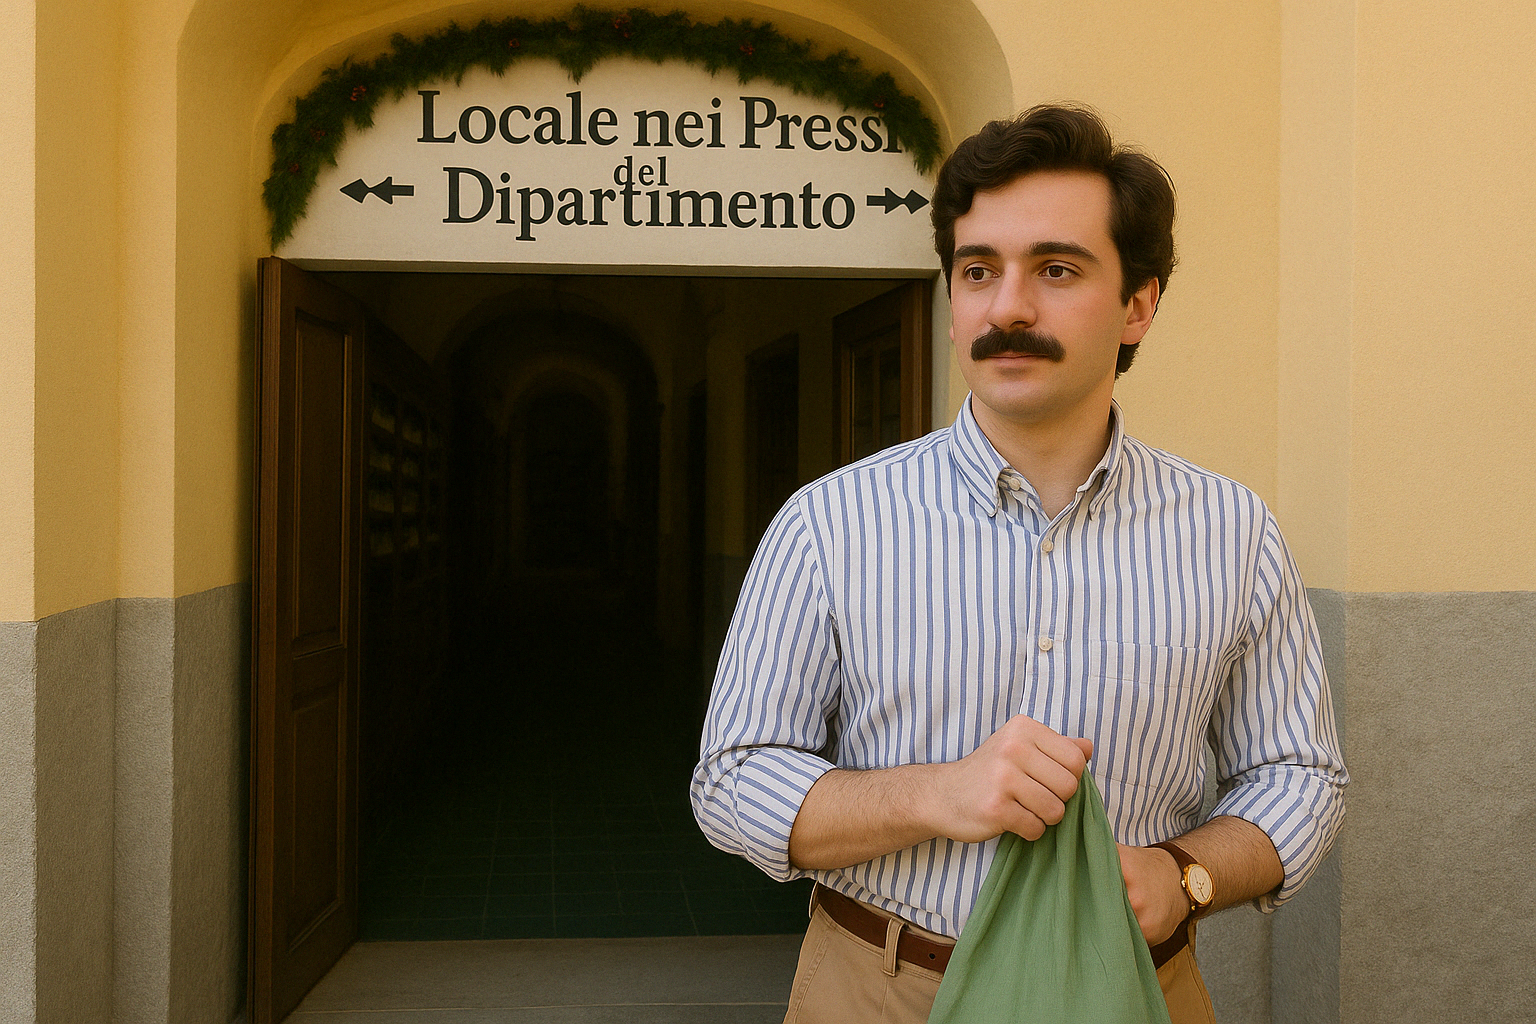
\includegraphics[width=\linewidth]{mirko.png}
\end{figure}
\end{frame}

\begin{frame}{Why psychometrics? The case of Dr. Mirko Marmellata}
\begin{block}{Dr. Marmellata}
every day chooses to buy lunch at the \textit{Place near the Department}, despite spending much more than bringing lunch from home, and never being completely satisfied with the quality and quantity offered.
\end{block}
\vspace{1em}
\begin{block}{By the standards of homo oeconomicus}
his choice would be \textbf{irrational}. To be kind, the choice still appears \textbf{non-optimal} to us.
\end{block}
\end{frame}

\begin{frame}{Why psychometrics? The case of Dr. Mirko Marmellata}
\begin{block}{Random Utility Model (RUM)}
\[
U_{ia} = V_{ia} + \varepsilon_{ia}
\]
\begin{itemize}
  \item \(U_{ia}\): total utility that individual \(i\) associates with alternative \(a\);
  \item \(V_{ia}\): observable component (price, quantity...);
  \item \(\varepsilon_{ia}\): unobserved component (habits, emotions...).
\end{itemize}
\end{block}
\vspace{1em}
\begin{block}{For Mirko Marmellata:}
\[
U_{\text{MM}, \text{Place}} > U_{\text{MM}, \text{Home}}
\]
What drives his preference is probably hidden in \(\varepsilon\).
\end{block}
\end{frame}

\begin{frame}{Why psychometrics? The case of Dr. Mirko Marmellata}
\begin{block}{The role of psychometrics}
It allows to ``open'' the \(\varepsilon\) and to model the latent constructs that influence decisions.
\end{block}
\vspace{1em}
\begin{block}{Objective}
Bring psychological factors out of \(\varepsilon\) and into the model, improving \textbf{prediction} and \textbf{understanding}.
\end{block}
\end{frame}

\section{Brief introduction to measurement theory}
\begin{frame}{Vietnam flashback...}
\begin{center}
   {\huge \alert{DATA GENERATING PROCESS}} 
\end{center}
\vspace{0.5cm}
\begin{itemize}
    \item How to measure something we cannot observe?
\end{itemize}
\pause
\vspace{0.5cm}
According to \textbf{measurement theory}, even if we cannot directly observe a theoretical concept (like intelligence), we can observe its {\it reflections} in reality: behaviors, responses, results... \\
\vspace{0.5 cm}
\footnotesize
{\it Example:} \\
We don't weigh a person's intelligence on a scale, but we can infer it from a series of signals: they graduated with honors, they are good with Stata, they use complicated words, they have read all the 19th-century Russian novels... {\it Note that much depends on our definition of intelligence!}
\end{frame}

\begin{frame}{What we mean by measurement}
\begin{block}{Proposed definition:}
    \textit{Systematic} assignment of a score to entities (individuals, objects, events...), such that the score represents a characteristic of those entities.
\end{block}
\pause
\begin{itemize}
    \item When the investigated characteristic is psychological in nature, the science of measurement is called \textbf{psychometrics}.
\end{itemize}
\end{frame}

\section{Constructs: conceptual and operational definitions}
\begin{frame}{Constructs}
Some characteristics of interest are simple to measure: consumer age, height, weight. \\ Others, like intelligence, self-esteem, or attitudes, cannot be observed directly.
\begin{itemize}
    \item These variables are called \textbf{constructs}.
\end{itemize}
\end{frame}

\begin{frame}{Constructs}
Constructs include (but are not limited to):
    \begin{itemize}
      \item Personality traits (e.g., extraversion)
      \item Emotional states (e.g., fear)
      \item Attitudes (e.g., toward certifications)
      \item Skills (e.g., in scientific subjects)
    \end{itemize}
\end{frame}

\begin{frame}{Constructs}
  \begin{itemize}
    \item The construct describes a \textit{general tendency} to act in a certain way, not a specific behavior in the moment.
    \item Constructs are \textbf{abstract syntheses} of complex processes.
    \item No single behavior or process can completely “define” the construct.
  \end{itemize}
\end{frame}

\begin{frame}{Conceptual definition of a construct}
  \begin{block}{What is a conceptual definition?}
    It describes the behaviors and internal processes that constitute a psychological construct, and explains how it relates to other variables.
  \end{block}
  \pause
  \begin{itemize}
    \item Example: \textbf{neuroticism} can be defined as the stable tendency to experience negative emotions (anxiety, anger, sadness) in multiple situations.
    \item It can also include: genetic origin, stability over time, correlations with physical pain and somatic symptoms.
    \pause
    \item Scientific definitions differ from dictionary ones (more precise, empirically testable, and open to revision).
    \item Often multiple conceptual definitions of the same construct exist in the literature.
  \end{itemize}
\end{frame}

\begin{frame}{Operational definition of a construct}
  \begin{block}{What is an operational definition?}
    It is a definition of a construct in terms of how it is concretely measured.
  \end{block}
  \pause
\vspace{0.8cm}
  \begin{center}
      \textbf{Conceptual definition} \\
      \bigskip
      $\Downarrow$ \quad \textit{\small Operationalization} \quad $\Downarrow$ \\
      \bigskip
      \textbf{Operational definition} \\
  \end{center}
\end{frame}

  
\begin{frame}{Operational definition of a construct}
  Operational measures are divided into three main categories:
  \begin{enumerate}
      \item \textbf{Self-report}: the individual reports their own thoughts, emotions, or behaviors.
      \item \textbf{Behavioral}: a behavior is observed and recorded.
      \item \textbf{Physiological}: biological processes are recorded.
    \end{enumerate}
\end{frame}

\begin{frame}{Example: Disgust response to an “expired\" yogurt}
\small
  Suppose we want to measure a consumer's \textbf{disgust} reaction to a yogurt that has passed its best-before date.
  \pause
      \begin{block}{Conceptual definition}
    Disgust is a basic emotion that manifests as an avoidance response to stimuli perceived as contaminating, infected, or degraded. It has an evolutionary function of protection from ingesting potentially dangerous substances.
  \end{block}
  \pause
    \begin{block}{Operational definitions}
  \begin{itemize}
    \item \textbf{Self-report}: the participant rates how disgusting they find the idea of tasting the product on a scale from 1 to 7.
    \item \textbf{Behavioral}: we observe if the participant refuses to taste the product.
    \item \textbf{Physiological}: we measure galvanic skin response (GSR) or facial muscle activity (EMG) related to disgust when we ask the participant to taste the product.
  \end{itemize}
\end{block}
\end{frame}

\section{Levels of measurement}
\begin{frame}{Levels of measurement}
  \begin{block}{The level of measurement can be:}
    \begin{enumerate}
      \item Nominal
      \item Ordinal
      \item Interval
      \item Ratio
    \end{enumerate}
 \end{block}
Each level communicates a different degree of quantitative information, and determines the appropriate statistical analyses.
\end{frame}

\begin{frame}{Nominal and Ordinal}
\begin{block}{Nominal}
    Category labels: e.g., gender, marital status, ethnicity, favorite color. \textbf{There is no order between the categories.}
\end{block}
\pause
\begin{block}{Ordinal}
    The categories have an order (e.g., “very satisfied”, “satisfied”, “dissatisfied”) \textbf{but it is not possible to assume that the distances between categories are equal.} \\
    \pause
    \centering
    \vspace{0.5em}
    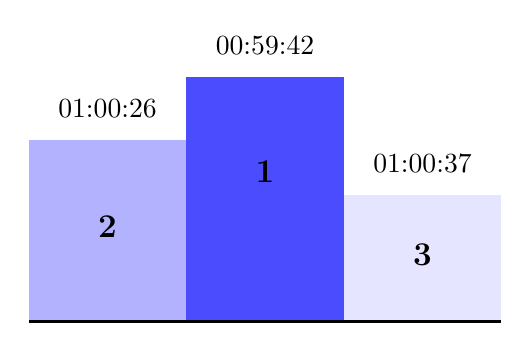
\begin{tikzpicture}[x=2cm,y=1cm]
  \fill[blue!30] (-1,-0.1) rectangle (0,2.2);     
  \fill[blue!70] ( 0,-0.1) rectangle (1,3.0);     
  \fill[blue!10] ( 1,-0.1) rectangle (2,1.5);     
  \node[font=\large\bfseries] at (-0.5,1.1) {2};
  \node[font=\large\bfseries] at ( 0.5,1.8) {1};
  \node[font=\large\bfseries] at ( 1.5,0.75) {3};
\draw[thick] (-1,-0.1) -- (2,-0.1);
    \pause
  \node at (-0.5,2.6) {01:00:26};
  \node at ( 0.5,3.4) {00:59:42};
  \node at ( 1.5,1.9) {01:00:37};
\end{tikzpicture}
\end{block}
\end{frame}

\begin{frame}{Interval and Ratio}
  \begin{block}{Interval}
  Numerical differences with consistent meaning: e.g., Celsius degrees. \\
  The distance between 12°C and 22°C is the same as that separating 22°C from 32°C. However...
    \begin{itemize}
      \item \textbf{No true zero:} 0°C does not mean “absence of temperature”.
      \item So \textbf{it makes no sense to speak of “double” or “half”:} 30°C is not twice as hot as 15°C.
    \end{itemize}
  \end{block}
  \pause
  \begin{block}{Ratio}
  Like interval, but with zero indicating the \textbf{absolute origin}. \\
    \begin{itemize}
      \item Allows for proportion comparisons: 100 kg is twice 50 kg.
      \item E.g.: height, weight, income, temperature in Kelvin.
    \end{itemize}
  \end{block}
\end{frame}

\begin{frame}{Recap}
    \centering
    Possible operations with different measurement scales: \\
    \vspace{1em}
    \begin{tabular}{lcccc}
    \toprule
      \textbf{Level} & \textbf{$=$ $\neq$} & \textbf{$>$ $<$} & \textbf{$+$ $-$} & \textbf{$\times$ $\div$} \\
      \midrule
      Nominal & \checkmark & & & \\
      Ordinal & \checkmark & \checkmark & & \\
      Interval & \checkmark & \checkmark & \checkmark & \\
      Ratio & \checkmark & \checkmark & \checkmark & \checkmark \\
      \bottomrule
    \end{tabular}
\end{frame}

\section{The questionnaire}
\begin{frame}{The second Copernican revolution?}
\huge
    \[
      \Delta x \cdot \Delta p_x \;\ge\; \frac{\hbar}{2}
    \]
\end{frame}

\begin{frame}{The second Copernican revolution?}
    \[
      \Delta x \cdot \Delta p_x \;\ge\; \frac{\hbar}{2}
    \]
\begin{block}{Uncertainty principle}
\small
    Enunciated by \textbf{Werner Heisenberg} in 1927, it represents a core concept of quantum mechanics and marked a radical break from the laws of classical mechanics. \\
    \smallskip
    We cannot know with absolute precision, simultaneously, the position and velocity of a particle: \textbf{the very act of measuring something changes it}. It is not a problem of imperfect instruments, but a fundamental characteristic of quantum nature.
\end{block}
\end{frame}

\begin{frame}{The questionnaire}
    The questionnaire is a \textbf{self-report} tool used to collect quantitative and/or qualitative information. Since it is generally completed independently by the participant, it can create the impression that the researcher is external to the process; in reality, the latter is solely responsible for the \\
    \vspace{1em}
    \pause
    \huge\centering
    \alert{DATA GENERATING PROCESS}
\end{frame}

\begin{frame}{The questionnaire}
\begin{block}{The participant}
    is not a database from which to extract data, but an \textbf{active subject} who uses various \textbf{contextual factors}, other than the content of the questions, to give meaning to the questionnaire they are completing. Some contextual effects: \\
    \begin{itemize}
        \item The way the questionnaire is presented.
        \item The identity of the researcher and the research institution.
        \item The response alternatives.
        \item The order of the questions.
    \end{itemize}
\end{block}
\end{frame}

\begin{frame}{Example: Order effect}
\textit{Strack et al. (1988) asked university students both how satisfied they were with their life in general and how often they went out on dates.} \\
\vspace{1em}
\centering
\begin{tabular}{l|lclc}
    \toprule
   Order 1 & Satisfaction & $\rightarrow$ & Dates & $r$ = -.12 \\
   \midrule
   \pause
   Order 2 & Dates & $\rightarrow$ & Satisfaction & $r$ = +.66 \\
   \bottomrule
\end{tabular}
\vspace{0.3cm}
\begin{block}{Possible solutions?}
\pause
\begin{itemize}
    \item \textbf{Space out} the questions in the questionnaire.
    \pause
    \item \textbf{Randomize} the presentation of the questions.
    \pause
    \item \textbf{Do both}.
\end{itemize}
\end{block}
\end{frame}

\begin{frame}{Cognitive processes in item response}
How many alcoholic drinks do you consume on a typical day? \\
\vspace{0.2cm}
\begin{tabular}{ll}
    $\bigcirc$ & Much more than average \\
    $\bigcirc$ & A bit more than average \\
    $\bigcirc$ & Average \\
    $\bigcirc$ & A bit less than average \\
    $\bigcirc$ & Much less than average \\
\end{tabular}
\vspace{1em}
\\ \textit{Even when we ask a seemingly trivial question, the response process can be complex, open to interpretations and manipulations.}
\end{frame}

\begin{frame}{Cognitive processes in item response}
  \resizebox{\textwidth}{!}{%
    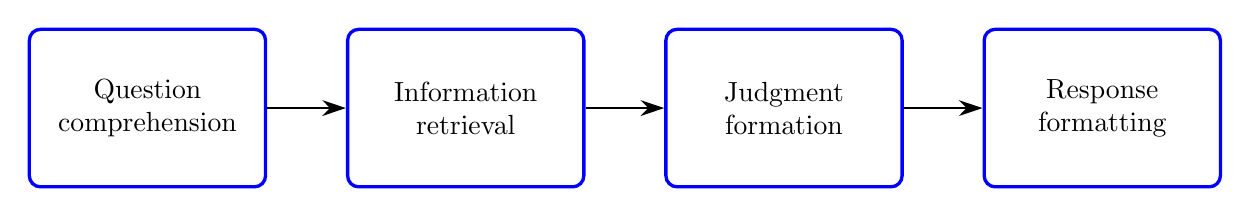
\begin{tikzpicture}[
      process/.style={
        rectangle, 
        draw=blue, very thick, 
        rounded corners, 
        minimum width=3cm, 
        minimum height=2cm, 
        align=center
      },
      arrow/.style={
        -{Stealth[length=3mm,width=2mm]}, 
        thick
      }
    ]
      \node[process] (comprehension) {Question \\ comprehension};
      \node[process, right=of comprehension] (retrieval) {Information \\ retrieval};
      \node[process, right=of retrieval] (judgment) {Judgment \\ formation};
      \node[process, right=of judgment] (response) {Response \\ formatting};
      \draw[arrow] (comprehension) -- (retrieval);
      \draw[arrow] (retrieval) -- (judgment);
      \draw[arrow] (judgment) -- (response);
    \end{tikzpicture}%
  }
\end{frame}

\begin{frame}{BORIS Model}
    The BORIS model\footnote{\scriptsize{Named BRUSO in \cite{jhangiani2019research}}} offers five useful principles for writing effective questionnaire questions.\\
    \vspace{1em}
    \begin{table}[]
        \centering
    \begin{tabular}{cc}
    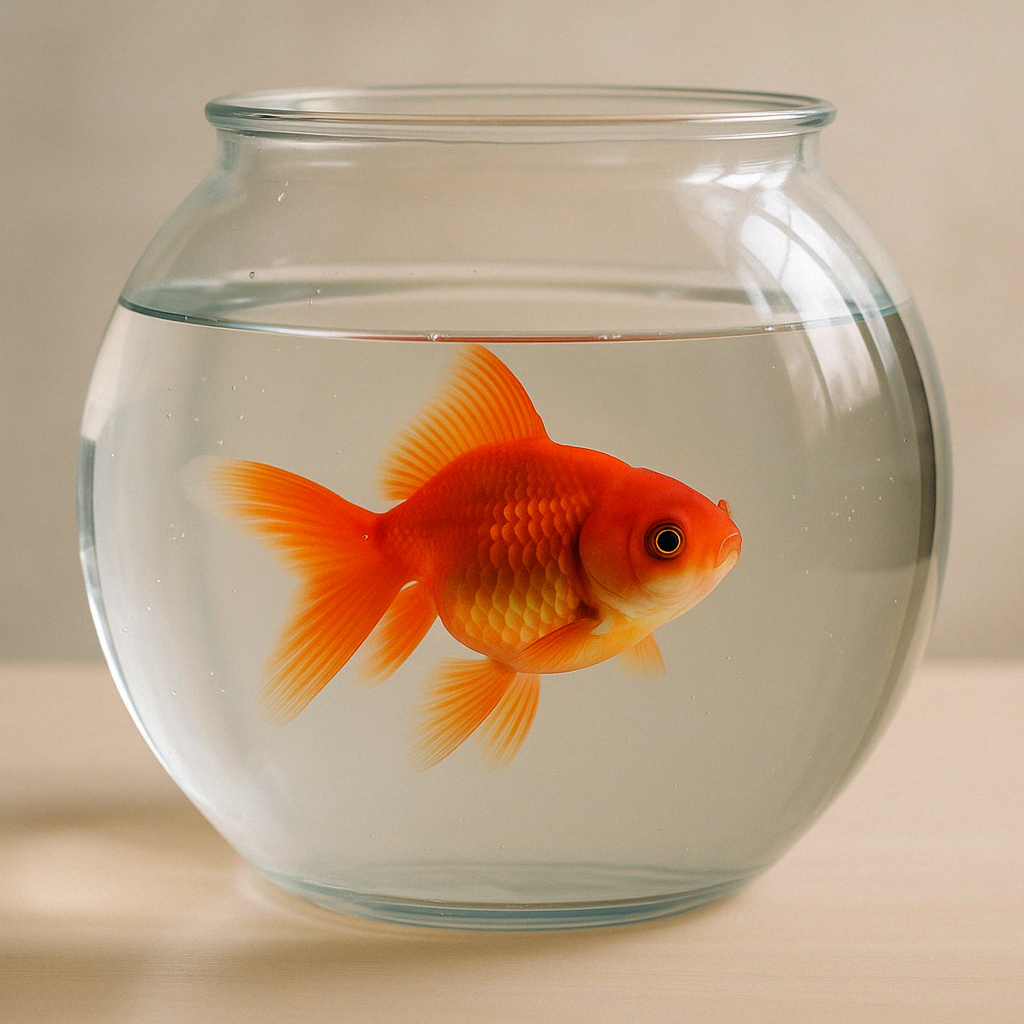
\includegraphics[width=0.45\linewidth]{boris.png} & 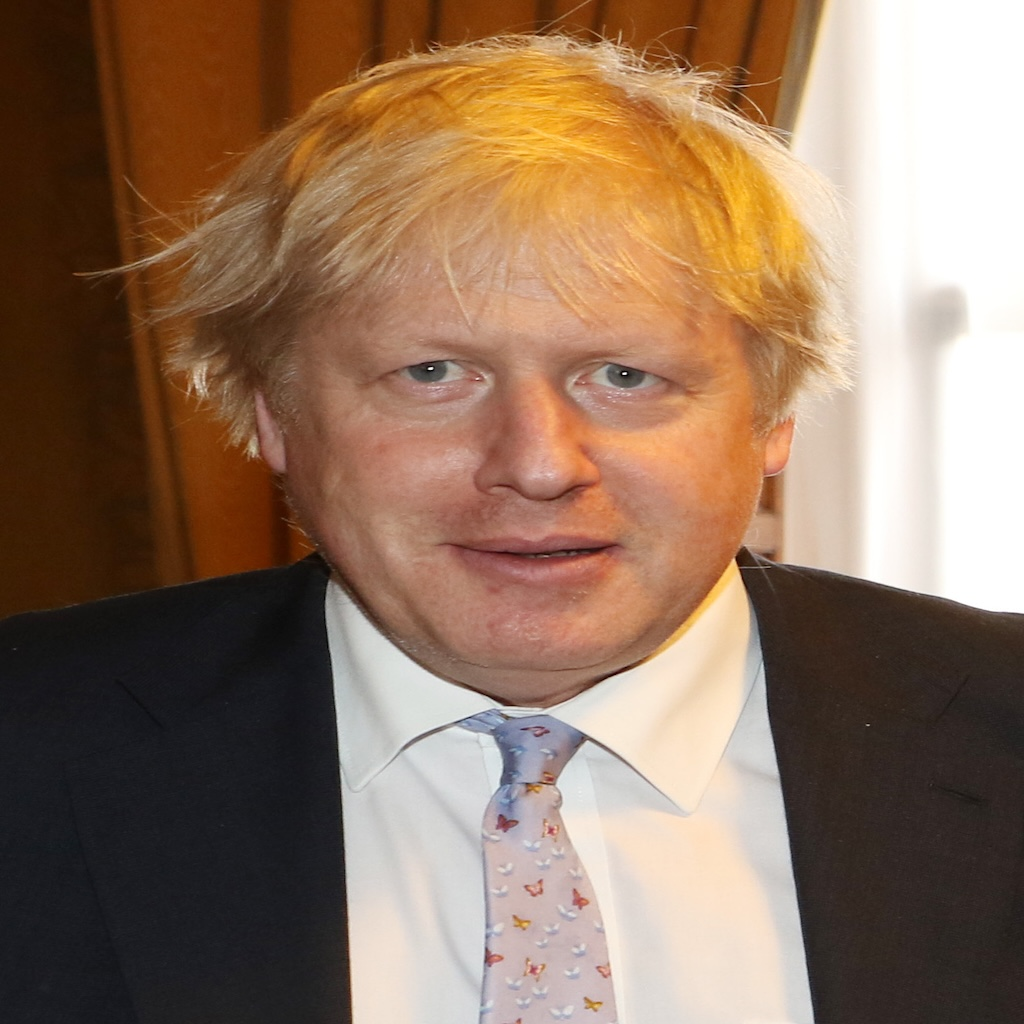
\includegraphics[width=0.45\linewidth]{boris2.jpg} \\
    \footnotesize{Goldfish} & \footnotesize{Former Prime Minister of the UK}
    \end{tabular}
    \end{table}
\end{frame}

\begin{frame}{BORIS Model}
  \scriptsize
  \centering
  \begin{tabular}{lp{4cm}p{3.5cm}}
    \toprule
    \textbf{Criterion} & \textbf{Less effective} & \textbf{OK} \\
    \midrule
    \textbf{B}revity & “Has it ever happened to you, in the course of your life, to come across the concept of social farming?” & “Have you ever heard of social farming?” \\
    \\
    \textbf{O}bjectivity & “How much do you support the NoCap ethical certification?” & “What is your opinion on the NoCap certification?” \\
    \\
    \textbf{R}elevance & “Which party did you vote for in the last political elections?” & Do not include the question if it is not clearly relevant. \\
    \\
    \textbf{I}nequivocality & “Are you a health-conscious person?” & “Do you habitually check nutritional labels when shopping?” \\
    \\
    \textbf{S}pecificity & “Have you ever heard of integrated production and SQNPI?” & “Have you ever heard of integrated production?” \\
    \bottomrule
  \end{tabular}
\end{frame}

\section{What are attitudes and how to measure them}
\begin{frame}{Attitudes $\neq$ Aptitudes}
    \begin{block}{What are attitudes?}
        Since 1918, over 500 definitions of attitudes have been coined! \\
        From the various definitions, a component of \textbf{evaluation} (positive-negative) of the subject with respect to an object emerges: \\
        \pause
        \small
    \begin{itemize}
        \item Allport (1954) defines attitude as a mental state, organized through experience, exerting an influence on the individual's responses to all objects and situations with which it is related.
        \item For Social Cognition (Fazio, 1986), attitude is a cognitive structure consisting of the association in memory between the representation of the object and its evaluation.
        \item Mayers (2021) defines attitude as a favorable or unfavorable evaluation toward something or someone, often rooted in one's beliefs and exhibited in feelings and intentional behavior.
    \end{itemize}
    \end{block}
\end{frame}

\begin{frame}{Attitudes $\neq$ Aptitudes}
    \begin{block}{What are attitudes for?}
        Katz (1960) suggests that attitudes can serve four main functions: \\
        \small
    \begin{enumerate}
        \item \textbf{Utilitarian}: the attitude toward a certain object develops to achieve a benefit or avoid a negative effect (e.g., positive attitude toward the vegan diet because it is perceived as healthier);
        \item \textbf{Value-expressive}: to express individual values and \textit{self-concept} (e.g., positive attitude toward the vegan diet to express one's \textit{ethical values});
        \item \textbf{Ego-defensive}: to defend a perceived lack at the identity level (e.g., negative attitude toward the vegan diet, by a man, because eating salad is not very manly); 
        \item \textbf{Knowledge}: to respond to the need for order, balance, and consistency...
    \end{enumerate}
    \end{block}
\end{frame}

\begin{frame}{Attitudes $\neq$ Aptitudes}
    \footnotesize
    \begin{block}{Balance Theory (Heider, 1946)}
        is based precisely on the principle of cognitive consistency, and formulates the existence of triadic attitudinal structures that tend toward cognitive restructuring in case of imbalance. \\
        The triadic structure is given by at least two people and at most one object. Depending on the attitudes with which they associate with each other, they can represent balanced or unbalanced structures that will, therefore, tend toward a change. \\
        \vspace{0.5em}
        \centering
        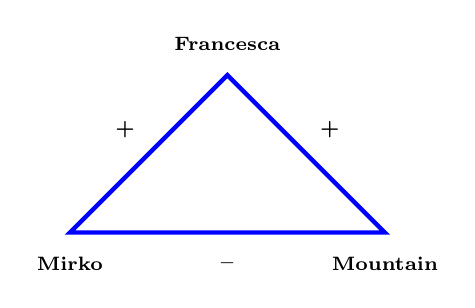
\begin{tikzpicture}
            \draw[blue, ultra thick] (4,0) -- (8,0) -- (6,2) -- cycle;
            \node at (4.7,1.3) {\textbf{\scriptsize+}};
            \node at (7.3,1.3) {\textbf{\scriptsize+}};
            \node at (6,-0.4) {\textbf{\scriptsize –}};
            \node at (4,-0.4) {\textbf{\scriptsize Mirko}};
            \node at (8,-0.4) {\textbf{\scriptsize Mountain}};
            \node at (6,2.4) {\textbf{\scriptsize Francesca}};
        \end{tikzpicture}
        \\
        \vspace{0.5em}
        \textit{\scriptsize A triad is considered in balance when the product of the signs is positive.} \\
    \end{block}
\end{frame}

\begin{frame}{Attitudes $\neq$ Aptitudes}
    \begin{block}{Balance Theory in marketing}
        Many companies use celebrity testimonials to promote the formation of a positive attitude toward their product or service.  \\
        \vspace{0.5em}
        \centering
        \pause
        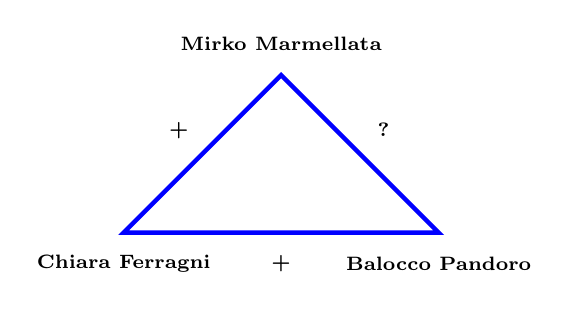
\begin{tikzpicture}
            \draw[blue, ultra thick] (4,0) -- (8,0) -- (6,2) -- cycle;
            \node at (4.7,1.3) {\textbf{\scriptsize +}};
            \node at (7.3,1.3) {\textbf{\scriptsize ?}};
            \node at (6,-0.4) {\textbf{\scriptsize +}};
            \node at (4,-0.4) {\textbf{\scriptsize Chiara Ferragni}};
            \node at (8,-0.4) {\textbf{\scriptsize Balocco Pandoro}};
            \node at (6,2.4) {\textbf{\scriptsize Mirko Marmellata}};
        \end{tikzpicture}
    \end{block}
\end{frame}

\begin{frame}{Attitudes $\neq$ Aptitudes}
    \begin{block}{Some basic characteristics:}
        \small
        \begin{itemize}
            \item Attitudes are relatively permanent over time and across situations.
            \item Attitudes always imply a certain degree of abstraction and are generalizable to multiple situations, objects, or conditions.
            \item Attitudes always have social relevance because they influence the person's perception in relation to others, preferences, and behaviors.
        \end{itemize}
        \textbf{Attitude is therefore a useful means for predicting consumption behaviors.}
    \end{block}
\end{frame}

\tikzset{
  block/.style = {draw=blue!80, fill=blue!10, very thick, ellipse, minimum height=2cm, minimum width=3cm, align=center}, arrow/.style = {thick, ->, >=Stealth}
}

\begin{frame}{Theory of Reasoned Action (Fishbein \& Ajzen, 1975)}
\resizebox{\textwidth}{!}{%
\centering
\begin{tikzpicture}[node distance=1.5cm, auto]
  \node[] (pbc) {};
  \node[block, above=of pbc] (att) {Attitude \\ toward the \\ behavior};
  \node[block, below=of pbc] (ns) {Subjective \\ norms};
  \node[block, right=of pbc] (int) {Behavioral \\ intention};
  \node[block, right=of int] (beh) {Behavior};
  \draw[arrow] (att) -- (int);
  \draw[arrow] (ns)  -- (int);
  \draw[arrow] (int) -- (beh);
\end{tikzpicture}
}
\end{frame}

\begin{frame}{Theory of Planned Behavior (Ajzen, 1991)}
\resizebox{\textwidth}{!}{%
\centering
\begin{tikzpicture}[node distance=1.5cm, auto]
  \node[block] (pbc) {Perceived \\ behavioral \\ control};
  \node[block, above=of pbc] (att) {Attitude \\ toward the \\ behavior};
  \node[block, below=of pbc] (ns) {Subjective \\ norms};
  \node[block, right=of pbc] (int) {Behavioral \\ intention};
  \node[block, right=of int] (beh) {Behavior};
  \draw[arrow] (att) -- (int);
  \draw[arrow] (pbc) -- (int);
  \draw[arrow] (ns)  -- (int);
  \draw[arrow] (int) -- (beh);
\end{tikzpicture}
} \\
\vspace{1em}
\footnotesize\centering\it 63\% of the professors here have at least one publication based on TPB!
\end{frame}

\begin{frame}{Measuring attitudes: Likert Scale}
\begin{columns}[c]
  \column{0.55\textwidth}
  \begin{figure}
    \centering
    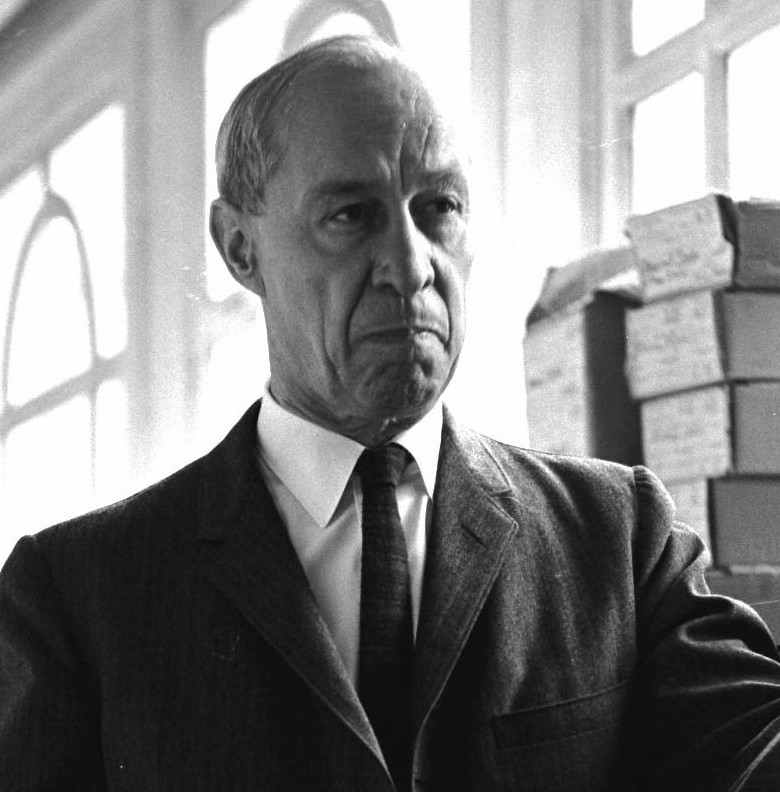
\includegraphics[width=\linewidth]{likert.jpg}
    \caption{Rensis Likert (1903–1981)}
  \end{figure}
  \column{0.45\textwidth}
  \begin{block}{Likert Scale}
    \small
    The Likert scale, or \textit{summated rating scale}, is widely used because it is easy to construct: a series of statements (\textit{items}) semantically linked to the attitudes to be studied are considered, and sets of questions are built on which the respondent is asked to express their degree of agreement or disagreement.
  \end{block}
\end{columns}
\end{frame}

\begin{frame}{Example: Food technology neophobia}
  \begin{block}{Food Technology Neophobia Scale (Cox \& Evans, 2008)}
    The FTNS is a popular tool for measuring food technology neophobia and is based on the Likert scale.
  \end{block}
  \vspace{0.3cm}
  \small
  \begin{tabular}{l l}
    \textbf{FTNS 1:} & I have no reason to try high-tech foods \\
    & because the ones I eat are already good enough \\
    \textbf{FTNS 2:} & New food technologies are something about which \\
    & I am uncertain \\
    \textbf{FTNS 3:} & New food products are not healthier than \\ 
    & traditional foods \\
    \textbf{(...)}
  \end{tabular}
  \vspace{0.2cm}
  \begin{center}
    \footnotesize
    \begin{tabular}{ccccc}
      \toprule
      \textit{Strongly} & \textit{Disagree} & \textit{Neither agree} & \textit{Agree} & \textit{Strongly} \\
      \textit{disagree} &  & \textit{nor disagree} &  & \textit{agree} \\
      \midrule
      $\bigcirc$ & $\bigcirc$ & $\bigcirc$ & $\bigcirc$ & $\bigcirc$ \\
      \bottomrule
    \end{tabular}
  \end{center}
\end{frame}

\begin{frame}{Example: Food technology neophobia}
  \begin{block}{Food Technology Neophobia Scale (Cox \& Evans, 2008)}
    The FTNS is a popular tool for measuring aversion toward new food technologies and is based on the Likert scale.
  \end{block}
  \vspace{0.3cm}
  \small
  \begin{tabular}{l l}
    \textbf{FTNS 1:} & I have no reason to try high-tech foods \\
    & because the ones I eat are already good enough \\
    \textbf{FTNS 2:} & New food technologies are something about which \\
    & I am uncertain \\
    \textbf{FTNS 3:} & New food products are not healthier than \\ 
    & traditional foods \\
    \textbf{(...)}
  \end{tabular}
  \vspace{0.2cm}
  \begin{center}
    \footnotesize
    \begin{tabular}{ccccc}
      \toprule
      \textit{Strongly} & \textit{Disagree} & \textit{Neither agree} & \textit{Agree} & \textit{Strongly} \\
      \textit{disagree} &  & \textit{nor disagree} &  & \textit{agree} \\
      \midrule
      1 & 2 & 3 & 4 & 5 \\
      \bottomrule
    \end{tabular}
  \end{center}
\end{frame}

\begin{frame}{Measuring attitudes: Semantic differential}
\begin{columns}[c]
  \column{0.55\textwidth}
  \begin{figure}
    \centering
    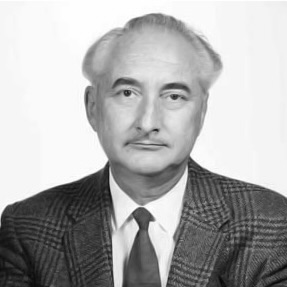
\includegraphics[width=\linewidth]{osgood.jpg}
    \caption{Charles E. Osgood (1916–1991)}
  \end{figure}
  \column{0.45\textwidth}
  \begin{block}{Osgood Scale}
    \small
    The Osgood scale, or \textit{semantic differential}, is based on pairs of opposite adjectives. The respondent indicates their position along a continuum, thus revealing their mental representation of the target concept.
  \end{block}
\end{columns}
\end{frame}

\begin{frame}{Example target: “Stata”}
  \begin{center}
    \small
    \begin{tabular}{|c|c|c|c|c|c|c|c|c|}
    \hline
      & -3 & -2 & -1 & 0 & 1 & 2 & 3 & \\
      \hline
      \text{Aggressive} & $\bigcirc$ & $\bigcirc$ & $\bigcirc$ & $\bigcirc$ & $\bigcirc$ & $\bigcirc$ & $\bigcirc$ & \text{Peaceful} \\
      \hline
      \text{Unpleasant}  & $\bigcirc$ & $\bigcirc$ & $\bigcirc$ & $\bigcirc$ & $\bigcirc$ & $\bigcirc$ & $\bigcirc$ & \text{Pleasant} \\
      \hline
      \text{...} & $\bigcirc$ & $\bigcirc$ & $\bigcirc$ & $\bigcirc$ & $\bigcirc$ & $\bigcirc$ & $\bigcirc$ & \text{...} \\
      \hline
    \end{tabular}
  \end{center}
  \pause
  \begin{figure}
    \centering
    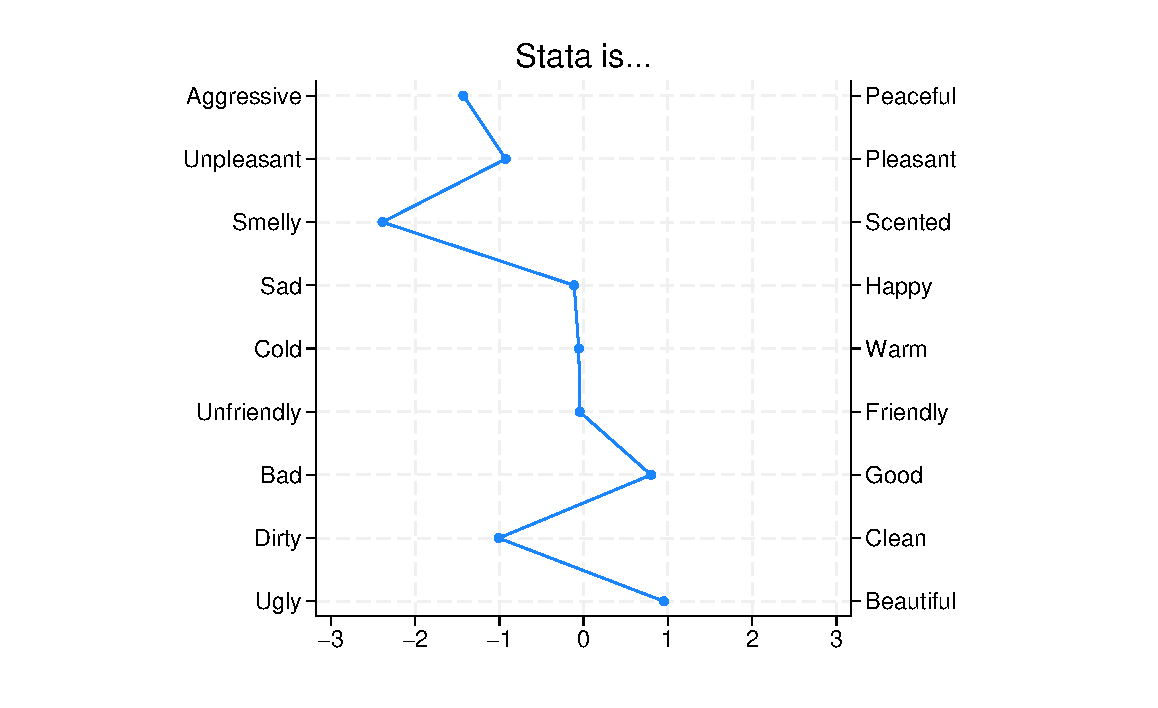
\includegraphics[width=0.9\linewidth]{osgood_en.eps}
  \end{figure}
\end{frame}

\end{document}
